% Created by tikzDevice version 0.12.3.1 on 2022-09-02 16:25:58
% !TEX encoding = UTF-8 Unicode
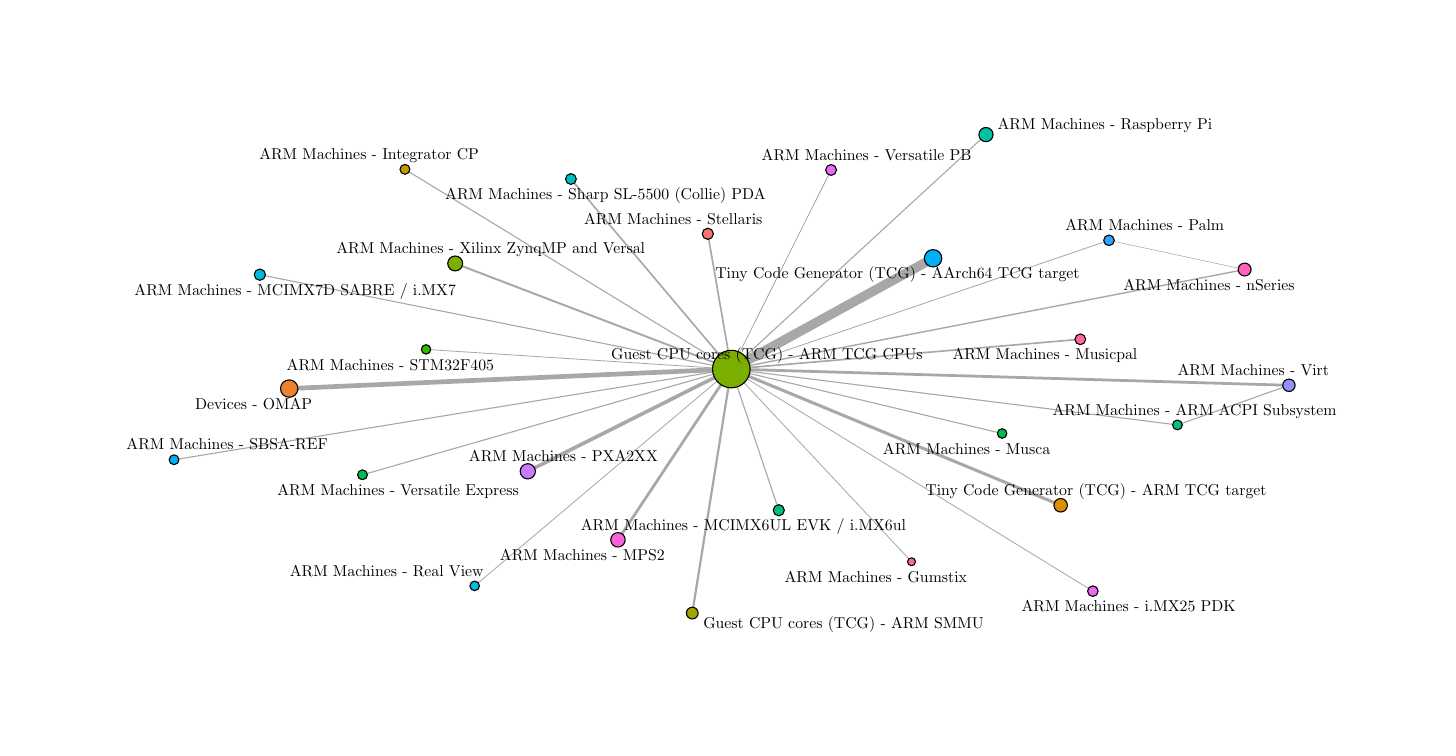
\begin{tikzpicture}[x=1pt,y=1pt]
\definecolor{fillColor}{RGB}{255,255,255}
\path[use as bounding box,fill=fillColor,fill opacity=0.00] (0,0) rectangle (505.89,252.94);
\begin{scope}
\path[clip] (  0.00,  0.00) rectangle (505.89,252.94);
\definecolor{fillColor}{RGB}{255,255,255}

\path[fill=fillColor] (  0.00,  0.00) rectangle (505.89,252.94);
\end{scope}
\begin{scope}
\path[clip] ( 32.75, 32.75) rectangle (475.89,222.94);
\definecolor{drawColor}{gray}{0.66}

\path[draw=drawColor,line width= 0.4pt,line join=round] (415.46,109.39) -- (455.75,123.71);

\path[draw=drawColor,line width= 0.4pt,line join=round] (415.46,109.39) -- (254.26,129.57);

\path[draw=drawColor,line width= 0.3pt,line join=round] (319.37, 59.95) -- (254.26,129.57);

\path[draw=drawColor,line width= 0.4pt,line join=round] (136.32,201.75) -- (254.26,129.57);

\path[draw=drawColor,line width= 0.4pt,line join=round] (271.41, 78.56) -- (254.26,129.57);

\path[draw=drawColor,line width= 0.4pt,line join=round] ( 83.89,163.69) -- (254.26,129.57);

\path[draw=drawColor,line width= 1.0pt,line join=round] (213.30, 67.88) -- (254.26,129.57);

\path[draw=drawColor,line width= 0.4pt,line join=round] (352.10,106.30) -- (254.26,129.57);

\path[draw=drawColor,line width= 0.6pt,line join=round] (380.37,140.33) -- (254.26,129.57);

\path[draw=drawColor,line width= 1.3pt,line join=round] (180.72, 92.63) -- (254.26,129.57);

\path[draw=drawColor,line width= 0.2pt,line join=round] (390.73,176.10) -- (439.75,165.54);

\path[draw=drawColor,line width= 0.3pt,line join=round] (390.73,176.10) -- (254.26,129.57);

\path[draw=drawColor,line width= 0.4pt,line join=round] (346.28,214.30) -- (254.26,129.57);

\path[draw=drawColor,line width= 0.3pt,line join=round] (161.52, 51.23) -- (254.26,129.57);

\path[draw=drawColor,line width= 0.4pt,line join=round] ( 52.89, 96.81) -- (254.26,129.57);

\path[draw=drawColor,line width= 0.3pt,line join=round] (143.95,136.68) -- (254.26,129.57);

\path[draw=drawColor,line width= 0.6pt,line join=round] (196.29,198.25) -- (254.26,129.57);

\path[draw=drawColor,line width= 0.6pt,line join=round] (245.76,178.46) -- (254.26,129.57);

\path[draw=drawColor,line width= 0.4pt,line join=round] (120.98, 91.37) -- (254.26,129.57);

\path[draw=drawColor,line width= 0.3pt,line join=round] (290.31,201.52) -- (254.26,129.57);

\path[draw=drawColor,line width= 1.0pt,line join=round] (455.75,123.71) -- (254.26,129.57);

\path[draw=drawColor,line width= 0.7pt,line join=round] (154.48,167.74) -- (254.26,129.57);

\path[draw=drawColor,line width= 0.3pt,line join=round] (384.90, 49.32) -- (254.26,129.57);

\path[draw=drawColor,line width= 0.5pt,line join=round] (439.75,165.54) -- (254.26,129.57);

\path[draw=drawColor,line width= 1.7pt,line join=round] ( 94.50,122.53) -- (254.26,129.57);

\path[draw=drawColor,line width= 0.8pt,line join=round] (240.15, 41.40) -- (254.26,129.57);

\path[draw=drawColor,line width= 3.4pt,line join=round] (254.26,129.57) -- (327.16,169.61);

\path[draw=drawColor,line width= 1.1pt,line join=round] (254.26,129.57) -- (373.27, 80.36);
\definecolor{drawColor}{RGB}{0,0,0}
\definecolor{fillColor}{RGB}{0,191,125}

\path[draw=drawColor,line width= 0.4pt,line join=round,line cap=round,fill=fillColor] (415.46,109.39) circle (  1.77);
\definecolor{fillColor}{RGB}{255,106,152}

\path[draw=drawColor,line width= 0.4pt,line join=round,line cap=round,fill=fillColor] (319.37, 59.95) circle (  1.43);
\definecolor{fillColor}{RGB}{192,155,0}

\path[draw=drawColor,line width= 0.4pt,line join=round,line cap=round,fill=fillColor] (136.32,201.75) circle (  1.79);
\definecolor{fillColor}{RGB}{0,191,125}

\path[draw=drawColor,line width= 0.4pt,line join=round,line cap=round,fill=fillColor] (271.41, 78.56) circle (  2.01);
\definecolor{fillColor}{RGB}{0,186,224}

\path[draw=drawColor,line width= 0.4pt,line join=round,line cap=round,fill=fillColor] ( 83.89,163.69) circle (  2.04);
\definecolor{fillColor}{RGB}{250,98,219}

\path[draw=drawColor,line width= 0.4pt,line join=round,line cap=round,fill=fillColor] (213.30, 67.88) circle (  2.61);
\definecolor{fillColor}{RGB}{0,187,78}

\path[draw=drawColor,line width= 0.4pt,line join=round,line cap=round,fill=fillColor] (352.10,106.30) circle (  1.72);
\definecolor{fillColor}{RGB}{255,106,152}

\path[draw=drawColor,line width= 0.4pt,line join=round,line cap=round,fill=fillColor] (380.37,140.33) circle (  1.94);
\definecolor{fillColor}{RGB}{199,124,255}

\path[draw=drawColor,line width= 0.4pt,line join=round,line cap=round,fill=fillColor] (180.72, 92.63) circle (  2.75);
\definecolor{fillColor}{RGB}{53,162,255}

\path[draw=drawColor,line width= 0.4pt,line join=round,line cap=round,fill=fillColor] (390.73,176.10) circle (  1.91);
\definecolor{fillColor}{RGB}{0,193,163}

\path[draw=drawColor,line width= 0.4pt,line join=round,line cap=round,fill=fillColor] (346.28,214.30) circle (  2.56);
\definecolor{fillColor}{RGB}{0,186,224}

\path[draw=drawColor,line width= 0.4pt,line join=round,line cap=round,fill=fillColor] (161.52, 51.23) circle (  1.73);
\definecolor{fillColor}{RGB}{0,176,246}

\path[draw=drawColor,line width= 0.4pt,line join=round,line cap=round,fill=fillColor] ( 52.89, 96.81) circle (  1.77);
\definecolor{fillColor}{RGB}{57,182,0}

\path[draw=drawColor,line width= 0.4pt,line join=round,line cap=round,fill=fillColor] (143.95,136.68) circle (  1.70);
\definecolor{fillColor}{RGB}{0,191,196}

\path[draw=drawColor,line width= 0.4pt,line join=round,line cap=round,fill=fillColor] (196.29,198.25) circle (  1.95);
\definecolor{fillColor}{RGB}{248,118,109}

\path[draw=drawColor,line width= 0.4pt,line join=round,line cap=round,fill=fillColor] (245.76,178.46) circle (  2.02);
\definecolor{fillColor}{RGB}{0,187,78}

\path[draw=drawColor,line width= 0.4pt,line join=round,line cap=round,fill=fillColor] (120.98, 91.37) circle (  1.78);
\definecolor{fillColor}{RGB}{231,107,243}

\path[draw=drawColor,line width= 0.4pt,line join=round,line cap=round,fill=fillColor] (290.31,201.52) circle (  1.96);
\definecolor{fillColor}{RGB}{149,144,255}

\path[draw=drawColor,line width= 0.4pt,line join=round,line cap=round,fill=fillColor] (455.75,123.71) circle (  2.23);
\definecolor{fillColor}{RGB}{124,174,0}

\path[draw=drawColor,line width= 0.4pt,line join=round,line cap=round,fill=fillColor] (154.48,167.74) circle (  2.69);
\definecolor{fillColor}{RGB}{231,107,243}

\path[draw=drawColor,line width= 0.4pt,line join=round,line cap=round,fill=fillColor] (384.90, 49.32) circle (  1.91);
\definecolor{fillColor}{RGB}{255,98,188}

\path[draw=drawColor,line width= 0.4pt,line join=round,line cap=round,fill=fillColor] (439.75,165.54) circle (  2.33);
\definecolor{fillColor}{RGB}{234,131,49}

\path[draw=drawColor,line width= 0.4pt,line join=round,line cap=round,fill=fillColor] ( 94.50,122.53) circle (  3.14);
\definecolor{fillColor}{RGB}{163,165,0}

\path[draw=drawColor,line width= 0.4pt,line join=round,line cap=round,fill=fillColor] (240.15, 41.40) circle (  2.12);
\definecolor{fillColor}{RGB}{124,174,0}

\path[draw=drawColor,line width= 0.4pt,line join=round,line cap=round,fill=fillColor] (254.26,129.57) circle (  6.78);
\definecolor{fillColor}{RGB}{0,176,246}

\path[draw=drawColor,line width= 0.4pt,line join=round,line cap=round,fill=fillColor] (327.16,169.61) circle (  3.14);
\definecolor{fillColor}{RGB}{216,144,0}

\path[draw=drawColor,line width= 0.4pt,line join=round,line cap=round,fill=fillColor] (373.27, 80.36) circle (  2.44);

\node[text=drawColor,anchor=base,inner sep=0pt, outer sep=0pt, scale=  0.57] at (421.66,112.96) {ARM Machines - ARM ACPI Subsystem};

\node[text=drawColor,anchor=base,inner sep=0pt, outer sep=0pt, scale=  0.57] at (306.47, 52.45) {ARM Machines - Gumstix};

\node[text=drawColor,anchor=base,inner sep=0pt, outer sep=0pt, scale=  0.57] at (123.38,205.33) {ARM Machines - Integrator CP};

\node[text=drawColor,anchor=base,inner sep=0pt, outer sep=0pt, scale=  0.57] at (258.63, 71.08) {ARM Machines - MCIMX6UL EVK / i.MX6ul};

\node[text=drawColor,anchor=base,inner sep=0pt, outer sep=0pt, scale=  0.57] at ( 96.66,156.22) {ARM Machines - MCIMX7D SABRE / i.MX7};

\node[text=drawColor,anchor=base,inner sep=0pt, outer sep=0pt, scale=  0.57] at (200.45, 60.40) {ARM Machines - MPS2};

\node[text=drawColor,anchor=base,inner sep=0pt, outer sep=0pt, scale=  0.57] at (339.29, 98.84) {ARM Machines - Musca};

\node[text=drawColor,anchor=base,inner sep=0pt, outer sep=0pt, scale=  0.57] at (367.59,132.87) {ARM Machines - Musicpal};

\node[text=drawColor,anchor=base,inner sep=0pt, outer sep=0pt, scale=  0.57] at (193.59, 96.21) {ARM Machines - PXA2XX};

\node[text=drawColor,anchor=base,inner sep=0pt, outer sep=0pt, scale=  0.57] at (403.64,179.67) {ARM Machines - Palm};

\node[text=drawColor,anchor=base,inner sep=0pt, outer sep=0pt, scale=  0.57] at (389.29,216.01) {ARM Machines - Raspberry Pi};

\node[text=drawColor,anchor=base,inner sep=0pt, outer sep=0pt, scale=  0.57] at (129.73, 54.78) {ARM Machines - Real View};

\node[text=drawColor,anchor=base,inner sep=0pt, outer sep=0pt, scale=  0.57] at ( 72.09,100.37) {ARM Machines - SBSA-REF};

\node[text=drawColor,anchor=base,inner sep=0pt, outer sep=0pt, scale=  0.57] at (131.06,129.18) {ARM Machines - STM32F405};

\node[text=drawColor,anchor=base,inner sep=0pt, outer sep=0pt, scale=  0.57] at (208.78,190.97) {ARM Machines - Sharp SL-5500 (Collie) PDA};

\node[text=drawColor,anchor=base,inner sep=0pt, outer sep=0pt, scale=  0.57] at (233.28,181.83) {ARM Machines - Stellaris};

\node[text=drawColor,anchor=base,inner sep=0pt, outer sep=0pt, scale=  0.57] at (133.86, 83.88) {ARM Machines - Versatile Express};

\node[text=drawColor,anchor=base,inner sep=0pt, outer sep=0pt, scale=  0.57] at (303.16,205.08) {ARM Machines - Versatile PB};

\node[text=drawColor,anchor=base,inner sep=0pt, outer sep=0pt, scale=  0.57] at (442.88,127.29) {ARM Machines - Virt};

\node[text=drawColor,anchor=base,inner sep=0pt, outer sep=0pt, scale=  0.57] at (167.31,171.30) {ARM Machines - Xilinx ZynqMP and Versal};

\node[text=drawColor,anchor=base,inner sep=0pt, outer sep=0pt, scale=  0.57] at (397.84, 41.80) {ARM Machines - i.MX25 PDK};

\node[text=drawColor,anchor=base,inner sep=0pt, outer sep=0pt, scale=  0.57] at (426.87,158.06) {ARM Machines - nSeries};

\node[text=drawColor,anchor=base,inner sep=0pt, outer sep=0pt, scale=  0.57] at ( 81.63,115.06) {Devices - OMAP};

\node[text=drawColor,anchor=base,inner sep=0pt, outer sep=0pt, scale=  0.57] at (294.79, 35.77) {Guest CPU cores (TCG) - ARM SMMU};

\node[text=drawColor,anchor=base,inner sep=0pt, outer sep=0pt, scale=  0.57] at (267.13,133.13) {Guest CPU cores (TCG) - ARM TCG CPUs};

\node[text=drawColor,anchor=base,inner sep=0pt, outer sep=0pt, scale=  0.57] at (314.29,162.13) {Tiny Code Generator (TCG) - AArch64 TCG target};

\node[text=drawColor,anchor=base,inner sep=0pt, outer sep=0pt, scale=  0.57] at (386.04, 83.91) {Tiny Code Generator (TCG) - ARM TCG target};
\end{scope}
\end{tikzpicture}
